% SC3010 --- Chapter 5: Software Security
% No \documentclass --- this file is \include'd by main.tex (book class).
\chapter{Software Security: Buffer Overflows, Injection, and Hardening}
\label{ch:software}
\begin{quote}
\emph{``Software is the attacker's favourite battlefield: every unchecked input is an invitation.''} --- From memory corruption to injected code, the flaw is the same: trusting data as if it were control.
\end{quote}

\noindent\fbox{\parbox{\dimexpr\linewidth-2\fboxsep-2\fboxrule}{%
\textbf{From zero: what this chapter builds on.} We assume no prior security knowledge. We start from how a program lays out memory (the stack), what it means to ``overflow'' a buffer, and why treating user input as code is dangerous. Every attack is shown first as a picture and concrete input-output, then formalized, then hardened. No cryptography or OS prerequisite beyond Ch.~1 foundations.
}}

\section*{Learning Outcomes}
After this chapter you will be able to:
\begin{enumerate}[label=(L\arabic*)]
    \item explain the stack layout and how an unchecked copy overwrites the return address;
    \item construct a minimal buffer-overflow exploit and describe its payload structure;
    \item distinguish SQL injection and XSS (stored, reflected, DOM) with concrete payloads;
    \item explain stack canaries, ASLR, and DEP/W\textasciicircum X and how each blocks an exploit stage;
    \item apply input validation and safe-API principles to prevent injection and overflow.
\end{enumerate}

% ============================================================
\section{Why Software Fails: Trusting Data as Control}
\label{sec:why-software-fails}
Every program mixes \emph{data} (what the user typed) with \emph{control} (where to jump, what query to run, what script to render). The processor, the SQL engine, and the browser all fetch the next instruction from somewhere writable if the programmer was careless. Think of a paper form: the box for ``name'' is data, but if you write past the box and onto the ``approved'' checkbox, data has become control.

Formally, a \emph{software vulnerability} is a state where an input causes execution to diverge from the intended control-flow graph or access-control policy. The three families below are the classic instances: memory corruption (control hijack), SQL injection (query-structure hijack), and XSS (browser-script hijack).

A useful mental model: the program is an interpreter that reads two tapes, \emph{program} and \emph{input}. A vulnerability merges the tapes so input symbols are decoded as program symbols. Hardening separates them again.

\begin{definition}[Control vs.\ data]
\emph{Control data} determines what executes next (return addresses, function pointers, SQL parse tree, HTML parser state). \emph{Non-control data} only influences values. Attacks that corrupt control data are strictly more powerful than those that only leak values.
\end{definition}

% ============================================================
\section{Buffer Overflows: Overwriting the Stack}
\label{sec:buffer-overflow}
On x86-like call stacks the frame for a function contains, from low to high addresses: local buffers, saved frame pointer, and the \emph{return address} --- the address execution resumes after \texttt{return}. The stack grows toward lower addresses, but buffers fill upward, toward control data.

\begin{figure}[h]\centering
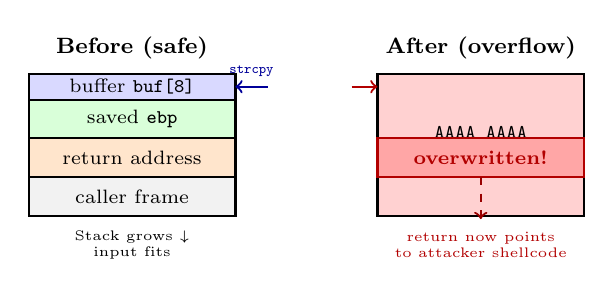
\begin{tikzpicture}[scale=0.82, every node/.style={font=\scriptsize}]
  % Before overflow
  \node[font=\footnotesize\bfseries] at (1.6,3.6) {Before (safe)};
  \draw[thick,fill=blue!15] (0,2.8) rectangle (3.2,3.2) node[midway] {buffer \texttt{buf[8]}};
  \draw[thick,fill=green!15] (0,2.2) rectangle (3.2,2.8) node[midway] {saved \texttt{ebp}};
  \draw[thick,fill=orange!20] (0,1.6) rectangle (3.2,2.2) node[midway] {return address};
  \draw[thick,fill=gray!10] (0,1.0) rectangle (3.2,1.6) node[midway] {caller frame};
  \draw[->,thick,blue!60!black] (3.7,3.0) -- (3.2,3.0) node[midway,above,font=\tiny] {\texttt{strcpy}};
  \node[font=\tiny,align=center] at (1.6,0.55) {Stack grows $\downarrow$\\input fits};
  % After overflow
  \node[font=\footnotesize\bfseries] at (7.0,3.6) {After (overflow)};
  \draw[thick,fill=red!18] (5.4,1.0) rectangle (8.6,3.2) node[midway,align=center,font=\scriptsize] {\texttt{AAAA AAAA}\\ \texttt{AAAA} + 0x080484b6};
  \draw[thick,fill=red!35,draw=red!70!black] (5.4,1.6) rectangle (8.6,2.2) node[midway,font=\scriptsize\bfseries,text=red!70!black] {overwritten!};
  \draw[->,thick,red!70!black] (5.0,3.0) -- (5.4,3.0);
  \node[font=\tiny,align=center,red!70!black] at (7.0,0.55) {return now points\\to attacker shellcode};
  \draw[->,thick,dashed,red!60!black] (7.0,1.6) -- (7.0,0.95);
\end{tikzpicture}
\caption{Stack frame before and after an overflow. An 8-byte buffer receives 18 bytes; the extra bytes overwrite the saved frame pointer and return address. Color shows corrupted region in red.}
\label{fig:stack-overflow}
\end{figure}

\begin{definition}[Buffer overflow]
A \emph{buffer overflow} occurs when a program writes $k$ bytes into a $b$-byte object with $k>b$ and without bounds checking, overwriting adjacent memory. If adjacent memory holds control data (return address, function pointer), the write is a \emph{control-flow hijack}.
\end{definition}

\begin{lstlisting}[language=C]
void vulnerable() {
    char buf[8];
    gets(buf);               // no length check -- NEVER use
    printf("echo: %s\n", buf);
}
int main(){ vulnerable(); return 0; }
\end{lstlisting}
Input \texttt{AAAAAAAAAAAA\textbackslash xb6\textbackslash x84\textbackslash x04\textbackslash x08} (12~As + little-endian address) overwrites the return address with \texttt{0x080484b6}. When \texttt{vulnerable} returns, \texttt{\%eip} jumps to the attacker address instead of \texttt{main}.

Exploit anatomy (intuition $\to$ formal):
\begin{enumerate}[label=(\alph*)]
    \item \emph{Overflow}: supply $b + \Delta$ bytes where $\Delta$ reaches the return slot.
    \item \emph{Payload}: shellcode or ROP gadgets placed in buffer or known library.
    \item \emph{Redirect}: overwritten return address $=$ payload address.
\end{enumerate}
Modern payloads avoid null bytes (which terminate \texttt{strcpy}) and use \emph{NOP sleds} (\texttt{\textbackslash x90} sled) to tolerate address imprecision: landing anywhere in the sled slides to shellcode.

\begin{example}[Off-by-one and 64-bit]
\texttt{for(i=0;i<=8;i++) buf[i]=input[i];} writes 9 bytes into \texttt{buf[8]}. On 32-bit little-endian this corrupts the saved \texttt{ebp} LSB, shifting the next frame. On 64-bit the canary and 8-byte addresses make exploitation harder but not impossible; ROP is the norm because stack is non-executable.
\end{example}

\begin{remark}[Heap and other targets]
Not every overflow hits the stack. Heap overflows corrupt heap metadata or adjacent objects (e.g., C++ vtables, function pointers in structs). The principle is identical: data written past its object reaches control data. We focus on the stack because it is the clearest illustration.
\end{remark}

% ============================================================
\section{Injection I: SQL Injection}
\label{sec:sqli}
Databases execute queries assembled by string concatenation. If user input is concatenated verbatim, it can escape the data context and become SQL syntax.

\begin{lstlisting}[language=Python]
# Vulnerable login (Python DB-API style)
query = "SELECT * FROM users WHERE name = '" + username + "' AND pw = '" + password + "'"
cursor.execute(query)
\end{lstlisting}

Attacker sets \texttt{username = \textquotesingle\ OR\ 1=1; --} yielding:
\begin{center}
\texttt{SELECT * FROM users WHERE name = '' OR 1=1; --' AND pw = ''} 
\end{center}
The \texttt{--} comments out the remainder; \texttt{1=1} is always true, so every row is returned --- authentication bypassed.

\begin{figure}[h]\centering
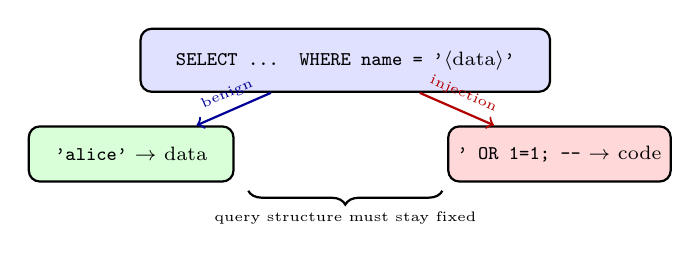
\begin{tikzpicture}[scale=0.85, every node/.style={font=\scriptsize}]
  \node[draw,thick,fill=blue!12,rounded corners,minimum width=5.2cm,minimum height=0.8cm] (q) at (0,1.4) {\texttt{SELECT ... WHERE name = '}$\langle$data$\rangle$\texttt{'}};
  \node[draw,thick,fill=green!15,rounded corners,minimum width=2.6cm,minimum height=0.7cm] (good) at (-3.2,0) { \texttt{'alice'} $\to$ data };
  \node[draw,thick,fill=red!15,rounded corners,minimum width=2.6cm,minimum height=0.7cm] (bad) at (3.2,0) { \texttt{' OR 1=1; --} $\to$ code };
  \draw[->,thick,blue!60!black] (q) -- (good) node[midway,above,sloped,font=\tiny] {benign};
  \draw[->,thick,red!70!black] (q) -- (bad) node[midway,above,sloped,font=\tiny] {injection};
  \draw[decorate,decoration={brace,mirror,amplitude=5pt},thick] (-1.45,-0.55) -- (1.45,-0.55) node[midway,below=4pt,font=\tiny] {query structure must stay fixed};
\end{tikzpicture}
\caption{SQL injection as breaking out of the data context. Benign input stays inside the quoted literal (blue$\to$green); attacker input escapes it and alters the query tree (red).}
\label{fig:sqli-context}
\end{figure}

\begin{definition}[SQL injection (SQLi)]
\emph{SQLi} is an injection where untrusted input is interpolated into a SQL statement without parameterisation, allowing the attacker to change the parse tree of the query.
\end{definition}

Blind and second-order variants exfiltrate data bit-by-bit (\texttt{AND SUBSTRING(pw,1,1)='a'}) or store payloads that fire later when an admin views them. The fix is invariant: never build SQL by string concatenation with untrusted data.

\begin{lstlisting}[language=Python]
# Safe: structure fixed, data bound separately (prepared statement)
cursor.execute("SELECT * FROM users WHERE name = ? AND pw = ?", (username, password))
# The template is compiled first; bindings are typed data, never parsed as SQL.
\end{lstlisting}

\begin{example}[UNION extraction]
With \texttt{cat=' UNION SELECT password FROM users--} the query becomes \texttt{SELECT id FROM products WHERE cat='' UNION SELECT password FROM users--}. The second SELECT appends password hashes to the product list, exfiltrating them in the normal response.
\end{example}

% ============================================================
\section{Injection II: Cross-Site Scripting (XSS)}
\label{sec:xss}
XSS injects JavaScript that the victim's browser executes in the origin of the vulnerable site --- stealing cookies, session tokens, or performing actions as the user. Unlike SQLi, the victim is the user, not the database.

\begin{description}[leftmargin=1.2em, itemsep=0.35em]\sloppy
    \item[Stored XSS] Payload is saved on the server (comment, profile) and served to every visitor. Example \lstinline[language=HTML,breaklines=true]!<script>alert(1)</script>! persists (the tag executes when the page is rendered).
    \item[Reflected XSS] Payload arrives in the request (e.g., \texttt{?q=<script>...}) and is echoed verbatim in the response. Needs a lure URL.
    \item[DOM XSS] No server reflection; client-side JS unsafely sinks attacker-controlled data into \texttt{innerHTML} or \texttt{eval}. Example: \texttt{el.innerHTML = location.hash.slice(1)}.
\end{description}\fussy

\begin{definition}[XSS]
\emph{Cross-Site Scripting} occurs when an application includes untrusted data in an HTML/JS context without proper output encoding, causing the browser to execute it as script in the application's origin.
\end{definition}

\begin{example}[Reflected payload]
Server echoes: \texttt{<p>Search: \$q</p>} without encoding. Attacker crafts \texttt{https://site/search?q=<svg onload=alert(1)>}. Victim clicks; browser parses \texttt{<svg...>} as active content. Stored variant: attacker posts a profile name \texttt{<img src=x onerror=alert(1)>} that every viewer executes.
\end{example}

Output encoding is context-sensitive: HTML-entity encode in element content, attribute-encode in attributes, JS-encode inside \texttt{<script>}. A single \texttt{htmlspecialchars} is not universally sufficient.
\begin{lstlisting}[language=Python]
# Context-aware encoding (Python illustration)
import html
safe_html = html.escape(user_input)          # for <div>content</div>
safe_attr = html.escape(user_input, quote=True)  # for <div title="...">
# For JS contexts use json.dumps; for URLs use urllib.parse.quote
\end{lstlisting}
Content Security Policy (CSP) adds a second layer: \texttt{Content-Security-Policy: script-src 'self'} blocks inline scripts even if an injection slips through.

% ============================================================
\section{Hardening: Canaries, ASLR, DEP, and Input Validation}
\label{sec:hardening}

No single defence suffices; they compose in layers. Each blocks a different stage of the exploit chain, from input entry to code execution.

\begin{figure}[h]\centering
\resizebox{\linewidth}{!}{%
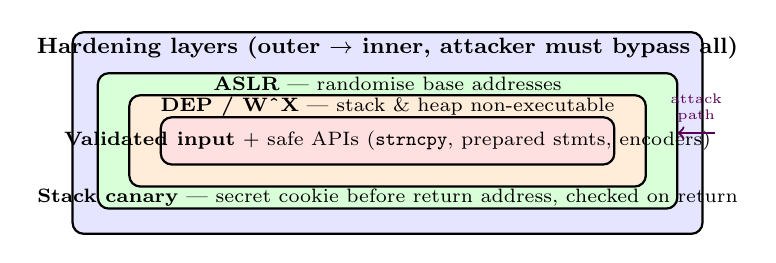
\begin{tikzpicture}[scale=0.80, every node/.style={font=\scriptsize}]
  \draw[thick,fill=blue!10,rounded corners] (0,0) rectangle (10,3.2);
  \node[font=\footnotesize\bfseries] at (5,2.95) {Hardening layers (outer $\to$ inner, attacker must bypass all)};
  \draw[thick,fill=green!15,rounded corners] (0.4,0.4) rectangle (9.6,2.55);
  \draw[thick,fill=orange!15,rounded corners] (0.9,0.75) rectangle (9.1,2.20);
  \draw[thick,fill=red!12,rounded corners] (1.4,1.10) rectangle (8.6,1.85);
  \node[align=center] at (5,1.48) {\textbf{Validated input} + safe APIs (\texttt{strncpy}, prepared stmts, encoders)};
  \node[align=center] at (5,2.02) {\textbf{DEP / W\textasciicircum X} --- stack \& heap non-executable};
  \node[align=center] at (5,2.38) {\textbf{ASLR} --- randomise base addresses};
  \node[align=center] at (5,0.58) {\textbf{Stack canary} --- secret cookie before return address, checked on return};
  \draw[->,thick,violet!70!black] (10.2,1.6) -- (9.6,1.6) node[midway,above,font=\tiny,align=center] {attack\\path};
\end{tikzpicture}}%
\caption{Defence in depth for memory and injection. Each layer blocks a different exploit stage; none alone is sufficient.}
\label{fig:hardening-layers}
\end{figure}

\begin{description}[leftmargin=1.2em, itemsep=0.35em]
    \item[Stack canaries] A random secret word is placed between buffer and return address. On function return the canary is checked; mismatch aborts via \texttt{\_\_stack\_chk\_fail}. Bypass requires leaking or brute-forcing the canary or corrupting elsewhere (e.g., heap, function pointer before the canary).
    \item[ASLR] Randomises base addresses of stack, heap, libraries on each run (and with PIE, the executable itself). Attacker cannot hard-code gadget addresses; needs an information leak or brute force (weak on 32-bit with only 8--16 bits of entropy; strong on 64-bit with 28+).
    \item[DEP / W\textasciicircum X] Marks data pages non-executable (NX bit); injected shellcode will fault on fetch. Bypass via \emph{return-oriented programming} (ROP): chain existing executable gadgets ending in \texttt{ret} to achieve arbitrary computation without injecting code.
    \item[Input validation] Allow-list validation: accept only known-good patterns (type, length, charset, range); reject or encode the rest. For memory, use bounds-checked APIs (\texttt{fgets}, \texttt{strlcpy}, \texttt{snprintf}, \texttt{gets} never); for SQL, prepared statements; for HTML, context-aware encoding and CSP.
\end{description}

Composition matters: canary stops linear overflows, ASLR stops address reuse, DEP stops code injection, validation stops the malformed input from entering at all. Together they force the attacker to chain multiple independent bypasses --- a leak to defeat ASLR, a ROP chain to defeat DEP, and a canary bypass to reach the return address.

\begin{theorem}[Layering principle]
No single hardening mechanism restores full memory safety; only their composition (plus safe languages or formal verification) approaches it. Each layer raises exploit cost by requiring an additional primitive (leak, write, execute).
\end{theorem}

\section{Exercises}
\label{sec:ch05-exercises}
\begin{enumerate}[label=E5.\arabic*, leftmargin=*, itemsep=0.6em]
    \item \textbf{Stack arithmetic.} A function has \texttt{char buf[16];} then saved \texttt{ebp} (4~B) then return address (4~B). (a) How many bytes must an input contain to overwrite the first byte of the return address? (b) If a 4~B canary is placed after \texttt{buf}, how many bytes to reach it, and what must the attacker do to avoid detection?
    \item \textbf{Exploit the C code.} Given the \texttt{vulnerable()} listing in \S\ref{sec:buffer-overflow}, craft a concrete 24-byte payload that overwrites the return address with \texttt{0x0804851a} on little-endian x86, explaining each segment (filler, canary if any, address bytes, null-byte issues).
    \item \textbf{SQLi construction.} A query is \texttt{SELECT id FROM products WHERE cat='\$cat' ORDER BY price}. Construct a payload for \texttt{\$cat} that (a) returns all rows, (b) extracts the first character of the admin password via a blind boolean condition, (c) propose the single-line fix using parameterised queries.
    \item \textbf{XSS taxonomy.} For each scenario classify as stored, reflected, or DOM XSS and give the precise sink: (a) comment \texttt{<b>\$name</b>} stored unescaped, (b) \texttt{?error=\$msg} echoed, (c) \texttt{location.hash} assigned to \texttt{innerHTML}. For (c) propose a safe alternative using \texttt{textContent}.
    \item \textbf{Defence bypass reasoning.} Explain why DEP alone does not stop ROP and why ASLR alone does not stop a leak-assisted attack. Describe a two-stage bypass that defeats DEP+ASLR together (information leak $\to$ ROP) and which additional layer (canary or validation) would block it earliest.
\end{enumerate}

\section*{Chapter Notes}
Aleph~One, ``Smashing the Stack for Fun and Profit'' (Phrack~49, 1996) is the canonical overflow introduction; modern defences are surveyed in Szekeres et al., ``SoK: Eternal War in Memory'' (Oakland~2013). SQLi taxonomy follows Halfond et al.~(2006); XSS contexts and encoders are detailed in OWASP Cheat Sheets and Klein (2005). For ROP see Shacham (CCS~2007). The hardening triad (canaries/StackGuard, ASLR/PaX, DEP/W\^{}X) is standard in all modern OSes and extended by Control-Flow Integrity (Abadi et al., 2005).

% End of Chapter 5
